\documentclass[border=2pt]{standalone}

% Drawing
\usepackage{tikz}

% Tikz Library
\usetikzlibrary{angles, quotes, decorations.markings}

%Styles

%%Arrow in the Middle
\tikzset{midarrow1/.style = {postaction=decorate, decoration={markings,mark=at position .24 with \arrow{stealth}}}}
\tikzset{midarrow2/.style = {postaction=decorate, decoration={markings,mark=at position .76 with \arrow{stealth}}}}
\tikzset{midarrow/.style={midarrow1,midarrow2}}

% Define Color
\definecolor{richelectricblue}{rgb}{0.03, 0.57, 0.82}
\definecolor{lust}{rgb}{0.9, 0.13, 0.13}

% Define Lengths
\def\X{4}
\def\Y{7.5}
\def\dY{0.6}
\def\dy{0.1}

\begin{document}
	
	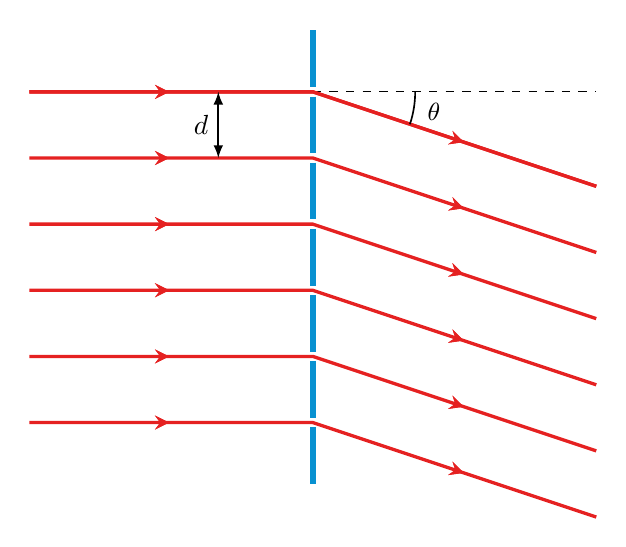
\begin{tikzpicture}[scale=1.2]
		% Grid
%		\draw[help lines] (0,0) grid (10,10);
		
		% Dashed Line
		\draw[dashed] (\X, \Y-\dY-\dy/2) coordinate(B) -- ++(3,0) coordinate(C); 
		
		% Slits	
		%% Top	
		\draw[line width = 2, color = richelectricblue] (\X,\Y) -- (\X, \Y-\dY) ;
		%% Bottom
		\draw[line width = 2, color = richelectricblue] (\X,\Y-6*\dY-6*\dy) -- (\X, \Y-6*\dY-\dY-6*\dy) ;
	
		% Slits And Rays
		\foreach \i in {0, ..., 5}
		{
			% Blue Walls
			\draw[line width = 2, color = richelectricblue] (\X,\Y-\i*\dY-\i*\dy) -- (\X, \Y-\i*\dY-\dY-\i*\dy) ;
			% Rays
			\draw[line width = 1.2, color = lust,  midarrow] (1, \Y-\i*\dY-\dY-\i*\dy-\dy/2) -- ++(\X-1, 0) -- ++(3, -1);
		}
		%% First Ray
		\draw[line width = 1.2, color = lust, angle eccentricity = 1.9] (1, \Y-\dY-\dy/2) -- ++(\X-1, 0) -- ++(3, -1) coordinate(A);
		
		%Angle
		\pic[line width = 0.6, draw, "\small$\theta$", black, angle radius=1.3cm, angle eccentricity = 1.2] {angle=A--B--C};
		
		% Node 
		\draw[line width = 0.6, black, latex-latex] (\X-1, 6.85) -- ++(0, -0.7) node [midway, left] {$d$};
	\end{tikzpicture}
	
\end{document}